
%(BEGIN_QUESTION)
% Copyright 2008, Tony R. Kuphaldt, released under the Creative Commons Attribution License (v 1.0)
% This means you may do almost anything with this work of mine, so long as you give me proper credit

If we take pressure measurements of fluid as it moves through a control valve and plot those pressures on a graph, we will get a curve that is highest at the upstream side ($P_1$), lowest at the point of maximum constriction in the valve ($P_{vc}$, the pressure at the {\it vena contracta}), and medium at the downstream side ($P_2$).  The following illustration shows three differently-constructed control valves, each with its own pressure profile:

$$\includegraphics[width=15.5cm]{i03254x01.eps}$$

Using the following equation to calculate {\it pressure recovery factor}, otherwise known as $F_L$, which of these three control valves exhibits the greatest pressure recovery factor value?

$$F_L = \sqrt{{P_1 - P_2} \over {P_1 - P_{vc}}}$$

\vfil 

\underbar{file i03254}
\eject
%(END_QUESTION)





%(BEGIN_ANSWER)

This is a graded question -- no answers or hints given!
 
%(END_ANSWER)





%(BEGIN_NOTES)

Valve \#3 has the greatest $F_L$ value, with $P_{vc}$ being greater than the other two valves, and both upstream and downstream pressures identical.

%INDEX% Mathematics review: qualitative algebra analysis

%(END_NOTES)


